\documentclass{beamer}

\usepackage[T2A,T1]{fontenc}
\usepackage[utf8]{inputenc}
\usepackage{biblatex}
\usepackage{hyperref}
\usepackage{blindtext}
\usepackage{wrapfig}
\usepackage{multicol}
\usepackage{xcolor}
\usepackage{graphicx}
\usepackage{setspace}
\usepackage{float}
\usepackage{newtxtext, newtxmath}
\usepackage{amsmath}

\addtobeamertemplate{navigation symbols}{}{%
    \usebeamerfont{footline}%
    \usebeamercolor[fg]{footline}%
    \hspace{1em}%
    \insertframenumber/\inserttotalframenumber
}

\graphicspath{ {./assets/} }
\bibstyle{plain}
\bibliography{references.bib}

\title{
	Topological and Geometric Deep Learning\\
	{\small Research Project}
}
\author{
	\textbf{Student}: Nikolay Chechulin, DSBA-201\\
	\textbf{Academic Supervisor}: Oleg Kachan, Research assistant at International Laboratory for Applied Topology and Applications
}
\institute{
	Data Science and Business Analytics\\
	Faculty of Computer Science\\
	
\includegraphics[height=.3\textheight]{assets/Higher_School_of_Economics_Logo.png}
}
\date{\today}

\begin{document}

\frame{\titlepage}

\section{Subject Area}

\begin{frame}
	\frametitle{\secname\ Overview}
	\tableofcontents[currentsection]
\end{frame}

\subsection{Clique}
\begin{frame}{\subsecname}
	A graph clique is a subset of its nodes such that it is fully connected.

	We will work mainly with 3-cliques, and often will refer to them as triangles.

	\begin{figure}[H]
		\centering
		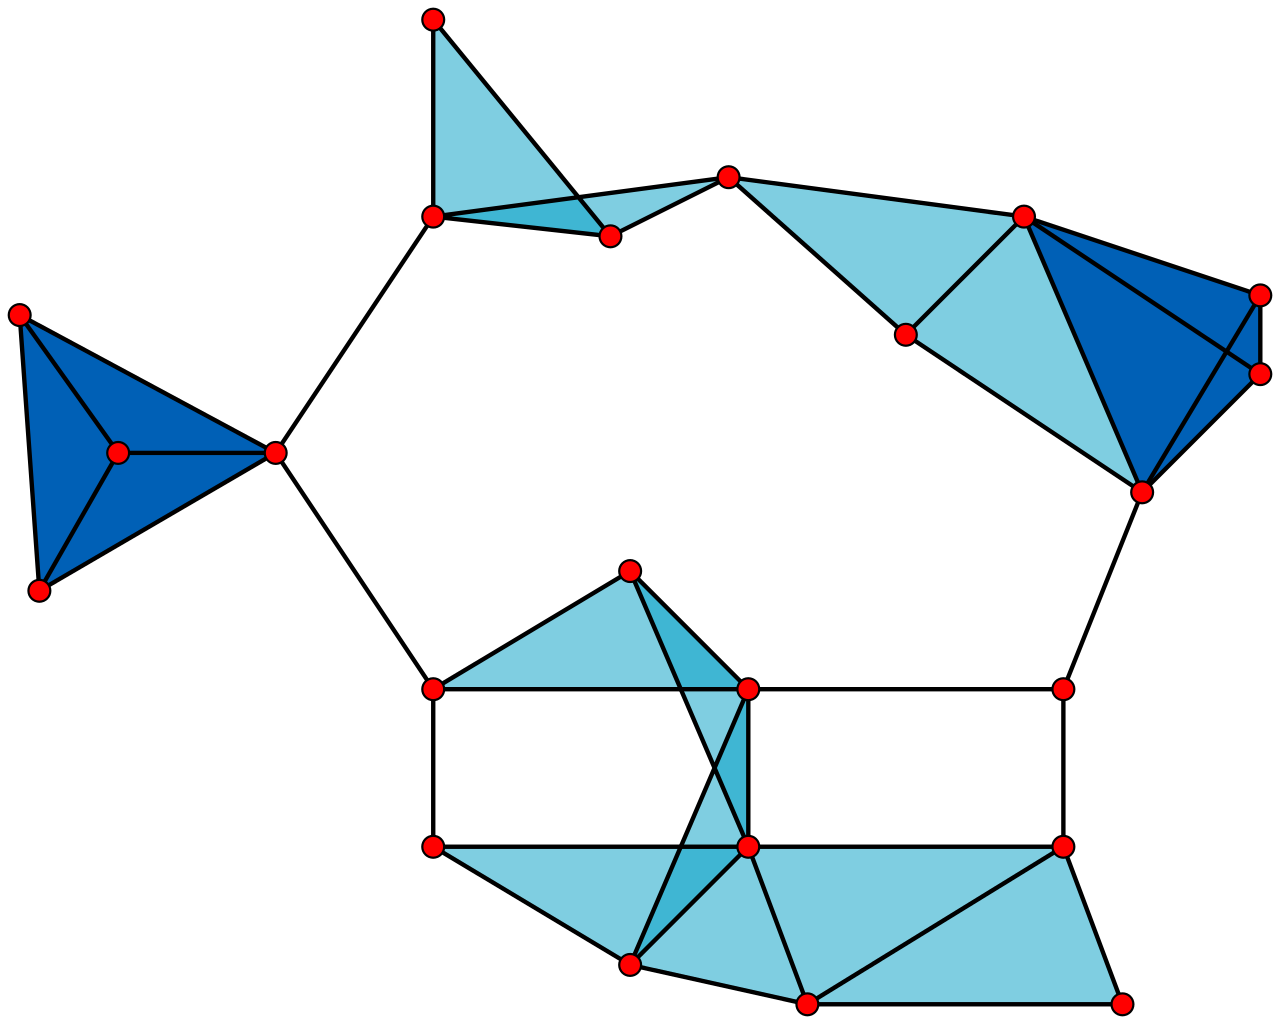
\includegraphics[height=0.6\textheight]{clique.png}
	\end{figure}
\end{frame}

%\subsection{Incidence Matrix}
%\begin{frame}{\subsecname}
%	If we have an undirected graph $(V, E)$, its incidence matrix $\nabla$ of size $\lvert V \rvert \times \lvert E \rvert$ such that $A_{i, j} = 1$ if $i$-th vertex is a vertex of $j$-th edge.
%	It shows relations between nodes and edges.

%	\begin{multicols}{2}
%		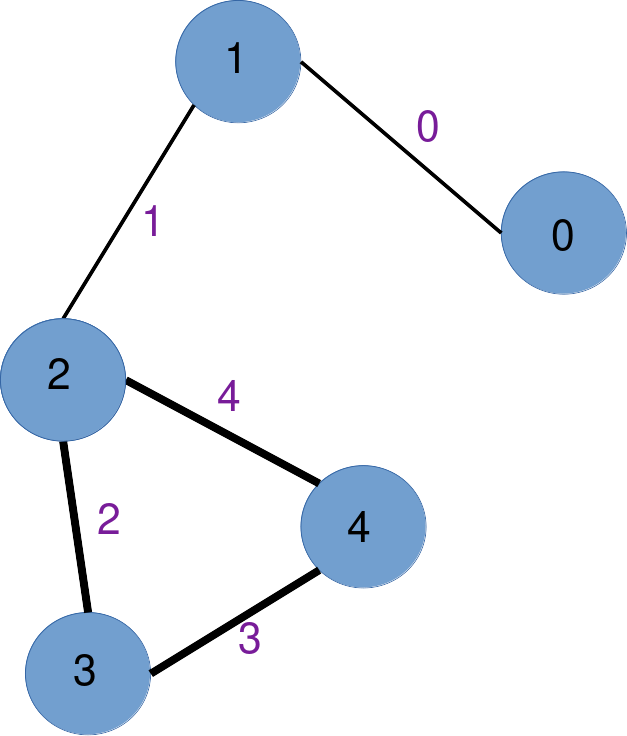
\includegraphics[width=0.3\textwidth]{incidence.png}

%		\[
%			\begin{bmatrix}
%				1 & 0 & 0 & 0 & 0 \\
%				1 & 1 & 0 & 0 & 0 \\
%				0 & 1 & 1 & 0 & 1 \\
%				0 & 0 & 1 & 1 & 0 \\
%				0 & 0 & 0 & 1 & 1 \\
%			\end{bmatrix}
%		\]

%	\end{multicols}
%\end{frame}

%\subsection{Laplacian matrix}
%\begin{frame}{\subsecname}
%	Another matrix representation of a graph.
%	Usually is calculated using the following formula:
%	\begin{equation*}
%		L_{i, j} =
%		\begin{cases}
%			\deg(v_i) & \mbox{if}\ i = j                                                 \\
%			-1        & \mbox{if}\ i \neq j\ \mbox{and}\ v_i \mbox{ is adjacent to } v_j \\
%			0         & \mbox{otherwise},
%		\end{cases}
%	\end{equation*}
%
%	However, other definitions also take place: $L = D - A$, where $D$ is a degree matrix and $A$ is an adjacency matrix.
%	Another way to calculate a Laplacian is $L = \nabla\nabla^{T}$, where $\nabla$ is an incidence matrix.
%\end{frame}

\subsection{Convolutional Graph Network}
\begin{frame}[allowframebreaks]{\subsecname}
	A type of GNN which generalizes the convolution operation to graphs.

	\begin{multicols}{2}
		\centering
		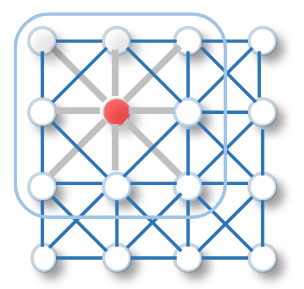
\includegraphics[width=0.4\textwidth]{conv.png}
		\caption{Convolution on image}
		\hfill
		\centering
		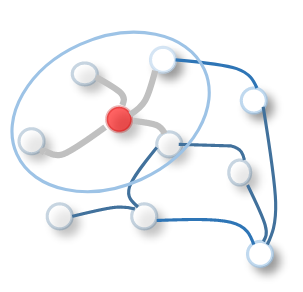
\includegraphics[width=0.4\textwidth]{CGN_conv.png}
		\caption{Convolution on graph}
	\end{multicols}

	\framebreak

	Assume we have a graph of $N$ nodes, where each node has $F$ features.
	We can construct an $N \times F$ matrix called feature matrix.
	The first layer takes the feature matrix, and performs the following operation: $Z = D^{-\frac{1}{2}} A D^{-\frac{1}{2}} X W$, where:
	\begin{itemize}
		\item $Z$ is resulting $N \times C$ signal
		\item $D$ is $N \times N$ degree matrix
		\item $A$ is $N \times N$ adjacency matrix with self-loops
		\item $X$ is $N \times F$ feature matrix (input signal)
		\item $W$ is $F \times C$ learnable weight matrix
	\end{itemize}

	The last (output) layer usually applies \emph{softmax} function to each row resulting in a new matrix $S$.
	Then, in order to classify a node $v_i$ we simply take the index of maximum of $S_i$.

	\framebreak

	The architecture of a graph convolutional network is presented on the figure below.
	\begin{figure}[h]
		\centering
		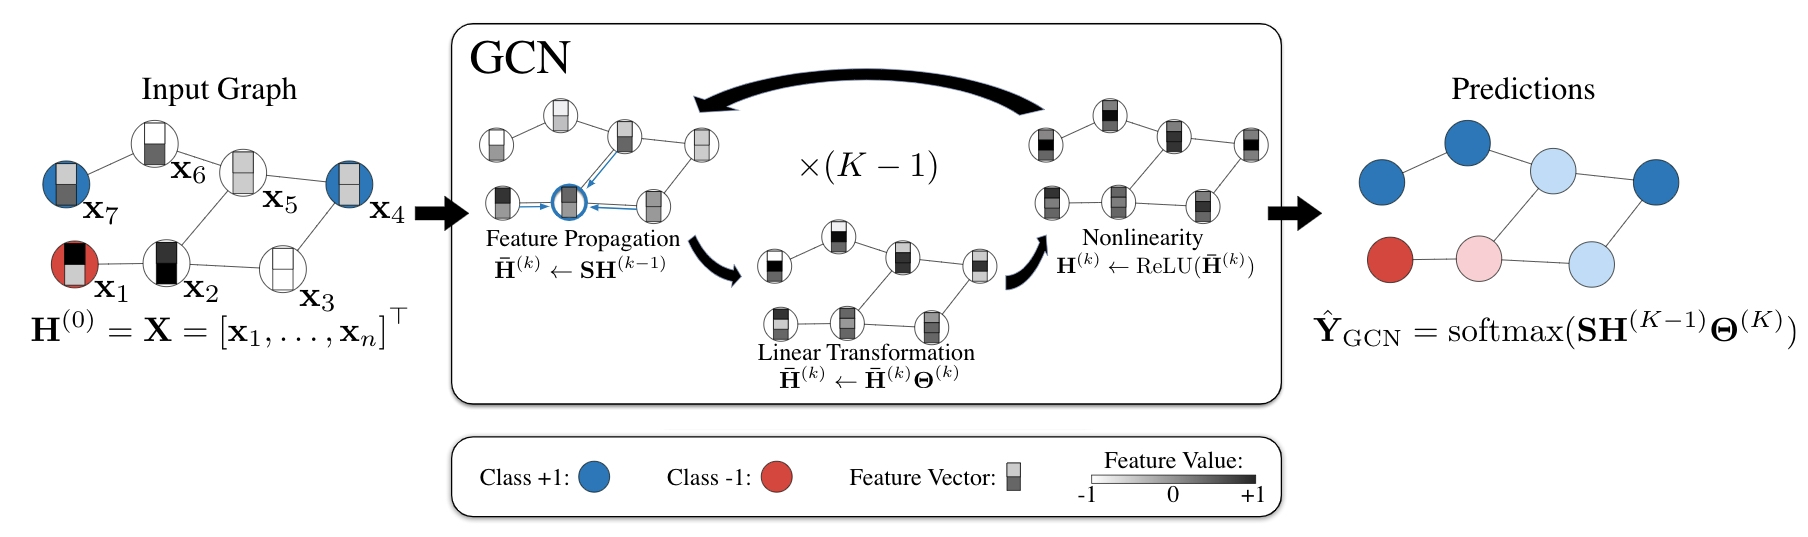
\includegraphics[width=\textwidth]{gcn.jpg}
	\end{figure}
\end{frame}

\subsection{Graph Attention Network}
\begin{frame}[allowframebreaks]{\subsecname}
	A type of GNN which uses attention mechanism (also borrowed from `casual' neural networks) which allows us to work with inputs of variable sizes and to focus on the most important features.
	The attention mechanism is a function $a: \mathbb{R}^C \times \mathbb{R}^C \rightarrow \mathbb{R}$ which takes two feature vectors $X_i, X_j$ and returns a scalar representing how tight the connection between $v_i$ and $v_j$ is.

	\framebreak

	We introduce an $N \times N$ matrix $e$ storing the attention between the nodes: $e_{i, j} = a\left( W \cdot X_i,\ W \cdot X_j \right)$.

	\textbf{Don't calculate all pairwise attentions!}
	One suggested solution is to use a neighborhood $\mathcal{N}_i$ of a vertex $v_i$ and then compute the attentions between $v_i$ and its' neighbors.
	Existing models uses neighborhood of size 1, and perform great.

	One might also want to normalize the coefficients.
	In order to do that, we can apply \empf{softmax} function: $c_{i, j} = \text{softmax}_j \left( e_{i, j} \right)$.

	\begin{figure}[h]
		\centering
		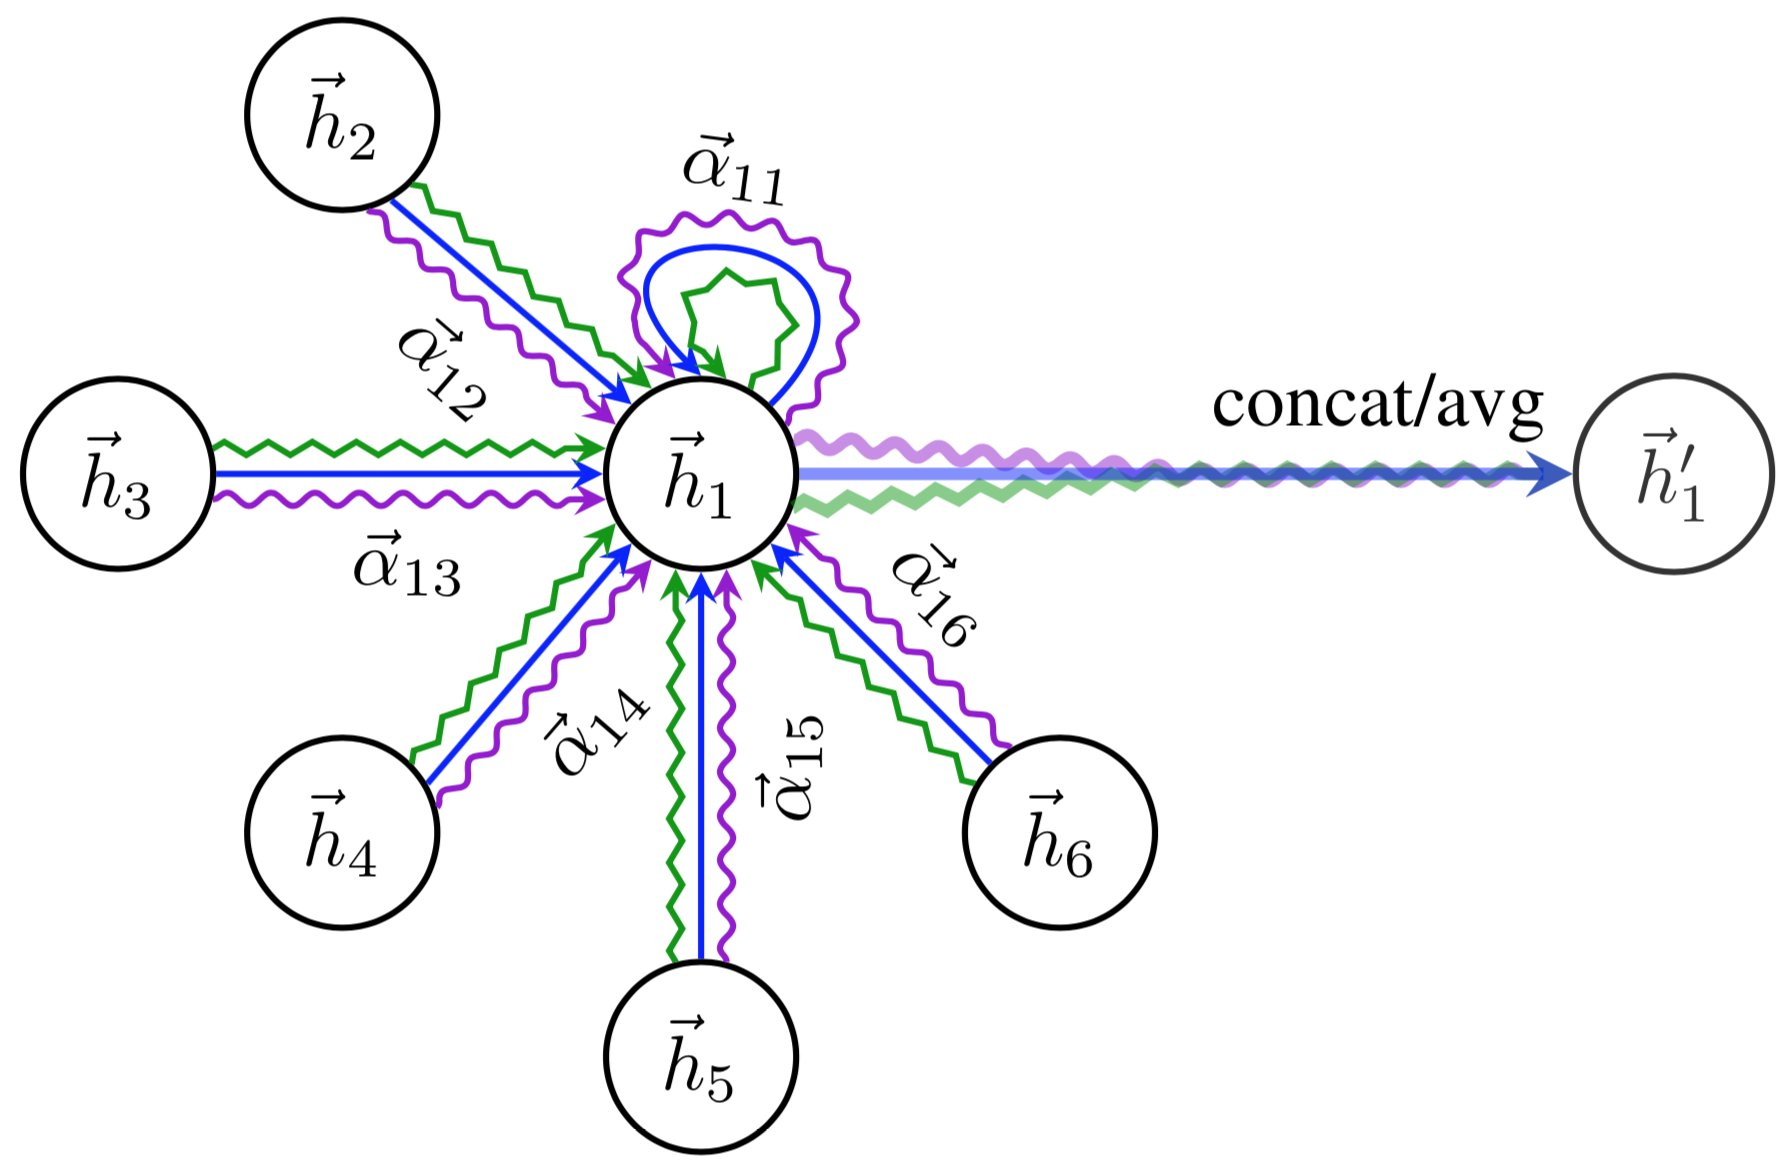
\includegraphics[width=0.7\textwidth]{gat.jpeg}
		\caption{An example of multi-head attention in a neighborhood of size 1}
	\end{figure}
\end{frame}

\subsection{Tasks solved by GNNs}
\begin{frame}{\subsecname}
	\begin{itemize}
		\item Node classification
		\item Graph classification
		\item Link prediction
	\end{itemize}
\end{frame}

\subsection{Purpose and objectives}
\begin{frame}{\subsecname}
	\begin{itemize}
		\item Study the foundation of Deep Learning models on graph data
		\item Research a few topological structures and methods
		\item Implement a topology-motivated preprocessing
		\item Conduct the experiments
	\end{itemize}
\end{frame}

\subsection{Relevance}
\begin{frame}{\subsecname}
	\begin{itemize}
		\item The field is new, therefore, there is a lot of space for improvement
		\item GNNs allow us to analyze complex relations with great precision
		\item We can improve the performance by preprocessing the data
		\item We can improve models by tweaking them
	\end{itemize}
\end{frame}


\section{Experiments and Results}

\begin{frame}
   \frametitle{\secname\ Overview}
   \tableofcontents[currentsection]
\end{frame}

\subsection{3-Clique merge with insertion}
\begin{frame}
	\frametitle{Method}
	Planetoid/Cora dataset:

	\begin{itemize}
		\item Node classification problem
		\item 2708 nodes
		\item 10556 edges
		\item 1433 features per node
		\item 5\% training node label rate
		\item 100 runs with 300 epochs
	\end{itemize}
\end{frame}

\begin{frame}{\subsecname\ Description}
	\begin{enumerate}
		\item Find all 3-cliques from a graph and save them in a list
		\item Sort them according to sum of pairwise distances
		\item Repeat the following steps until there are any nodes in a list:
			\begin{enumerate}
				\item Take the `top' 3-clique
				\item Save \emph{all} edges coming in/out of the clique
				\item Compute a `generic feature vector' by taking average of their feature vectors
				\item Delete them from the graph
				\item Create a new `merged' node with a generic feature vector and all saved edges
				\item Filter out the deleted nodes from list of 3-cliques
			\end{enumerate}
	\end{enumerate}
\end{frame}

\begin{frame}[allowframebreaks]
	\frametitle{3-clique Merge Example}

	The following figures show exactly how a 3-clique is merged: the resulting feature vector is the average of the feature vectors of initial nodes: $\frac{1}{3} \cdot \left( (1, 4, 5) + (2, 7, 1) + (0, 1, 6) \right) = \frac{1}{3} \cdot (3, 12, 12) = (1, 4, 4)$
	
	\begin{figure}[h]
		\begin{minipage}{.7\textwidth}
		  \centering
		  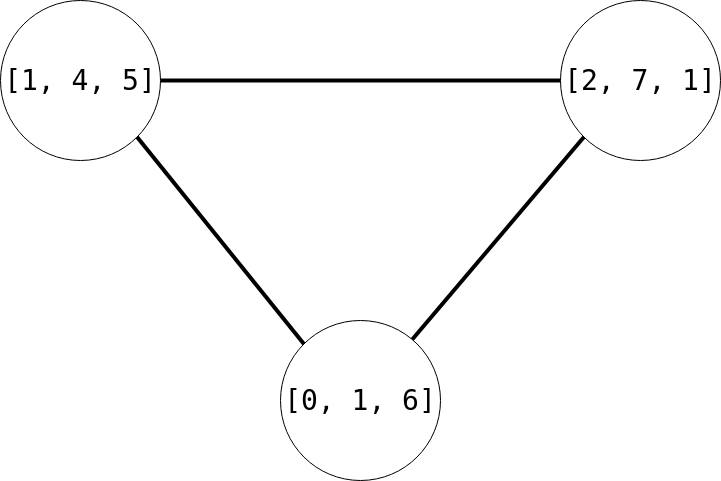
\includegraphics[width=0.8\linewidth]{3clique_before_merge_example}
		\end{minipage}%
		\begin{minipage}{.3\textwidth}
		  \centering
			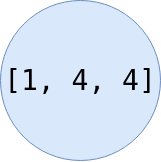
\includegraphics[width=0.6\linewidth]{3clique_merged_example}
		\end{minipage}
	\end{figure}
	
	\framebreak

  \begin{figure}[h]
	  \begin{multicols}{2}
		  \centering
		  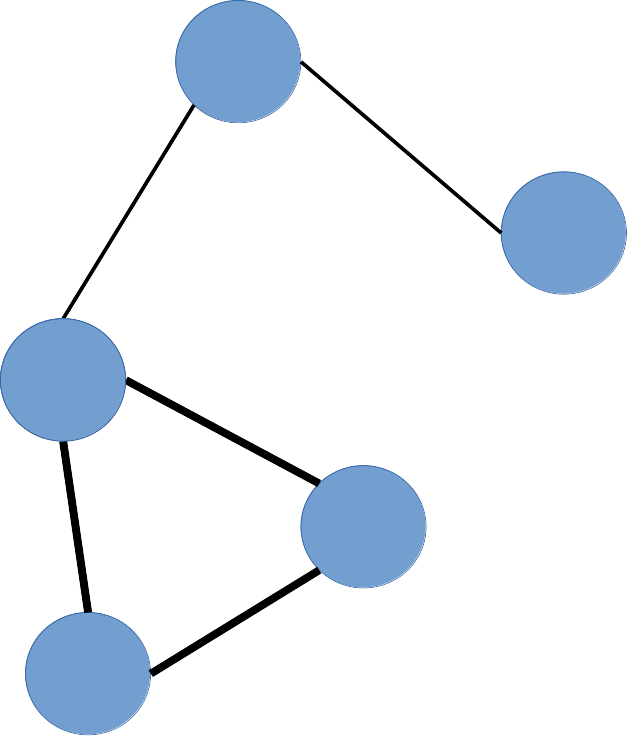
\includegraphics[width=0.4\textwidth]{simplex_1.png}
		  \caption{A part of some graph}\label{fig:clique_merged}

			\centering
			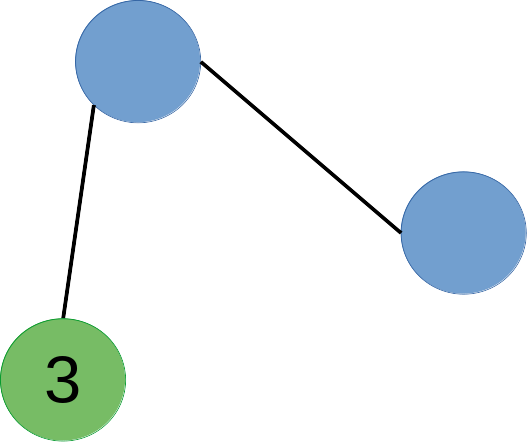
\includegraphics[width=0.4\textwidth]{simplex_2.png}
			\caption{Three nodes from the left image united in 3-simplex having properties of the initial vertices}
		\end{multicols}
	\end{figure}
\end{frame}

\begin{frame}[allowframebreaks]
	\frametitle{Results}
	
	\centering
	\begin{tabular}{ |c|c|c|c| }
		\hline
	 	Feature & Before & After & Delta \\
		\hline
		Node num & 2708 & 2120 & 21.71\% \\
		Edge num & 10556 & 4568 & 56.73\% \\
		Learning time & 4.171s & 2.939s & 29.5\% \\
		Accuracy & 0.803 & 0.746 & 7\% \\
	 \hline
	\end{tabular}

	\framebreak
	
	Accuracies graph:
	\begin{center}
		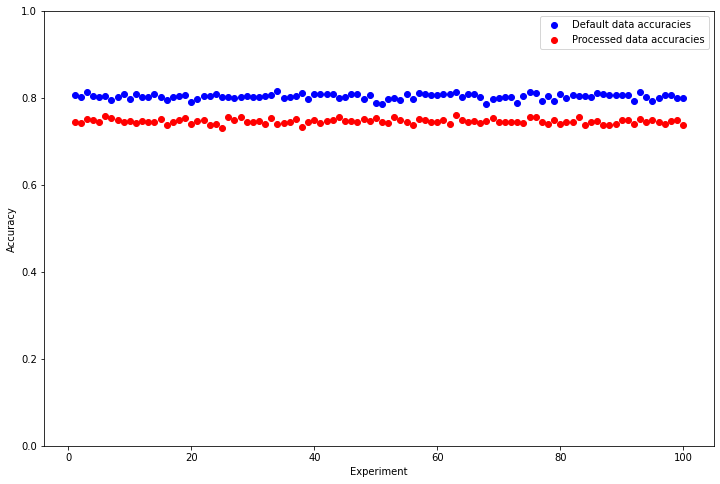
\includegraphics[width=\textwidth]{3clique_accuracy.png}
	\end{center}
\end{frame}

\subsection{Infinite 3-clique merge with insertion}

\begin{frame}{\subsecname\ Description}
	In this experiment, the methodology and the algorithm are similar to the `finite 3-clique merge'.
	The only difference is that we \emph{allow} merged nodes to participate in merge process again.
\end{frame}

\subsubsection*{Results and interpretation}
\begin{frame}[allowframebreaks]
	\frametitle{Results}
	The proposed method allowed us to remove the majority of information from a graph.

	\centering	
	\begin{tabular}{ |c|c|c|c| }
		\hline
	 	Feature & Before & After & Delta \\
		\hline
		Node num & 2708 & 1080 & 60.12\% \\
		Edge num & 10556 & 656 & 93.79\% \\
		Learning time & 2.537s & 1.059s & 58\% \\
		Accuracy & 0.809 & 0.517 & 36\% \\
	 \hline
	\end{tabular}

	\framebreak

	\begin{figure}[h]
		\centering
		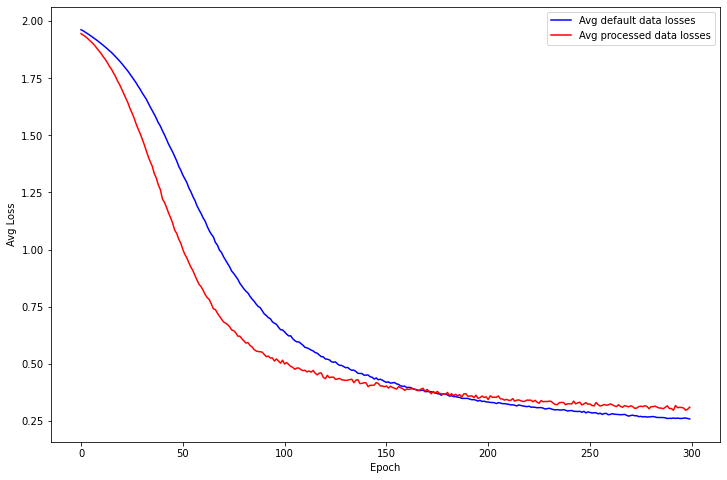
\includegraphics[width=\textwidth]{3clique_inf_loss}
		\caption{Average loss for `default' and processed data}
	\end{figure}

	\framebreak

	\begin{figure}[h]
		\centering
		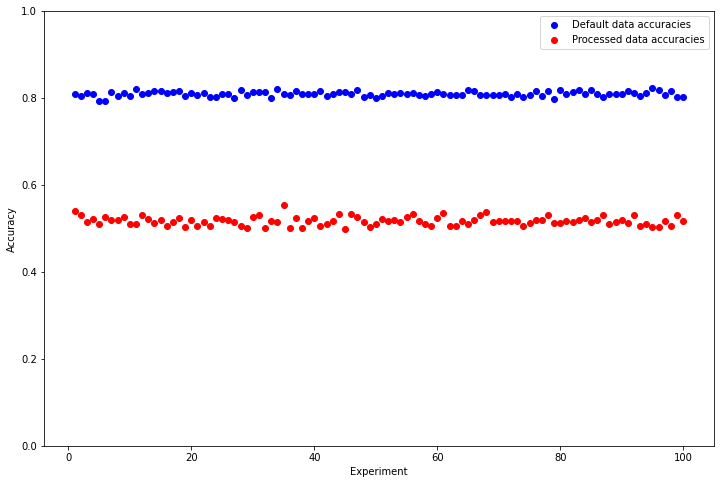
\includegraphics[width=\textwidth]{3clique_inf_accuracy}
		\caption{Accuracies of models with `default' and processed data}
	\end{figure}
\end{frame}

\subsection{Prospects}
\begin{frame}{\subsecname}
	In future we want to focus on topological aspect of the transformation presented in the paper.
	In particular, we are interested in `infinite merge', where `merged nodes' can be merged again.
	We also want to see how the transformation presented can be used in other tasks, for example, in graph classification.
\end{frame}


\begin{frame}[allowframebreaks]
	\frametitle{References}
	\nocite{*}
	\printbibliography{}
\end{frame}

\begin{frame}[plain, c]
	\begin{center}
		\Huge Any questions?
	\end{center}
\end{frame}

\end{document}

